\documentclass{article}
\usepackage{fullpage}
\usepackage{amsfonts}
\usepackage{amssymb}
\usepackage{amsmath}
\usepackage{hyperref}
\usepackage{graphicx}% Include figure files
\usepackage{epstopdf}
\usepackage{subfig}

%\usepackage{setspace}\doublespace
\author{Guojun Zhu}
\title{Narrow Feshbach Resonance}
\newcommand{\vk}{\ensuremath{\mathbf{k}}}
\providecommand{\vr}{\ensuremath{\mathbf{r}}}
%\newcommand{\vec}[1]{\ensuremath{\mathbf{#1}}}

\newcommand{\gk}{\ensuremath{{g}(\mathbf{k})}}

\newcommand{\vp}{\ensuremath{\mathbf{p}}}
\newcommand{\gp}{\ensuremath{{g}(\mathbf{p})}}

\newcommand{\vq}{\ensuremath{\mathbf{q}}}

\newcommand{\Fo}{\ensuremath{\mathbf{F_0}}}


\newcommand{\E}{\ensuremath{\mathbf{E}}}
\newcommand{\A}{\ensuremath{\mathbf{A}}}
\newcommand{\J}{\ensuremath{\mathcal{J}}}

\newcommand{\ket}[1]{\ensuremath{\left|#1\right>}}
\newcommand{\bra}[1]{\ensuremath{\left<#1\right|}}

\newcommand{\twoe}{\ensuremath{2\epsilon_\vk-\E_1}}

\newcommand{\nth}[1]{\ensuremath{\frac{1}{#1}}}

\newcommand{\br}[1]{\ensuremath{\left(#1\right)}}
\newcommand{\mbr}[1]{\ensuremath{\left[#1\right]}}
\newcommand{\bbr}[1]{\ensuremath{\left\{#1\right\}}}


\newcommand{\tk}{\ensuremath{\tilde{k}}}

\newcommand{\kp}{\ensuremath{\ket{\Psi}}}

\newcommand{\av}[1]{\ensuremath{\bigl<{#1}\bigr>}}
\newcommand{\avv}[2][\nu]{\av{#1{\lvert{#2}\rvert}#1}}
\newcommand{\avt}[2]{\av{{#1}|{#2}}}
\newcommand{\avtu}[1]{\av{T_\tau#1}}

\newcommand{\Bop}{\ensuremath{\mathbf{B_0^+}}}
\newcommand{\Bmp}{\ensuremath{\mathbf{B_m^+}}}
\newcommand{\Bnp}{\ensuremath{\mathbf{B_n^+}}}
\newcommand{\Bo}{\ensuremath{\mathbf{B_0}}}
\newcommand{\Bopn}{\ensuremath{\mathbf{{B_0^+}^n}}}
\newcommand{\Bon}{\ensuremath{\mathbf{{B_0}^n}}}


\newcommand{\zmatrix}{\ensuremath{\br{\begin{smallmatrix}0&0\\0&0\end{smallmatrix}}}}
\newcommand{\fmtrx}[4]{\ensuremath{\br{\begin{smallmatrix}#1&#2\\#3&#4\end{smallmatrix}}}}
\newcommand{\smtrx}[6]{\ensuremath{\br{\begin{smallmatrix}#1&#2\\#3&#4\\#5&#6\end{smallmatrix}}}}

\newcommand{\vz}{\ensuremath{v^{\beta\alpha}_{\vk,\vk}}}
%\newcommand{\fz}{

\providecommand{\abs}[1]{\ensuremath{\lvert{#1}\rvert}}

\newcommand{\sg}[1][1]{\ensuremath{\sigma_\frac{#1}{2}}}

\newcommand{\rhof}{\ensuremath{\rho(\ef)}}
\newcommand{\omt}{\ensuremath{\tilde{\Omega}}}
\newcommand{\cht}{\ensuremath{\tilde{\chi_0}}}
\newcommand{\Atl}{\ensuremath{\abs{A}^{2l}}}
\newcommand{\ef}{\ensuremath{\epsilon_F}}

\newcommand{\lca}{\ensuremath{\ln\br{1+\frac{\cht}{\alpha}}}}

\newcommand{\com}[2]{\ensuremath{\mbr{#1,#2}}}
\newcommand{\D}{\ensuremath{\mathit{D}}}
\newcommand{\dg}{\ensuremath{\dagger}}

\providecommand{\lvk}{\ensuremath{1/\vk_F}}
\providecommand{\hm}{\ensuremath{\frac{\hbar^2}}{2m}}
\providecommand{\pdiff}[2]{\ensuremath{\frac{\partial{#1}}{\partial{#2}}}}
\providecommand{\dpdiff}[2]{\ensuremath{\frac{\partial^2{#1}}{\partial{{#2}^2}}}}

\providecommand{\H}{\ensuremath{\mathcal{H}}}
\providecommand{\wt}[1]{\widetilde{#1}}

\renewcommand{\emph}[1]{\textbf{#1}}
\begin{document}
\maketitle

%\tableofcontents
\numberwithin{equation}{section}
\section{}
 The full two-channel hamiltonian is
\begin{equation}\label{eq:uvw:hamiltonian}
\begin{split}
 H=&\sum_\vk\epsilon^a_\vk{}a^+_\vk{}a^{}_\vk+\sum_\vk\epsilon^b_\vk{}b^+_\vk{}b^{}_\vk+\sum_\vk\epsilon^c_\vk{}c^+_\vk{}c^{}_\vk\\
  &+\nth{2}\sum_{\vk\vk'}U_{\vk\vk'}a^+_\vk{}b^+_{-\vk}{}b^{}_{-\vk'}a^{}_{\vk'}
	+\nth{2}\sum_{\vk\vk'}V_{\vk\vk'}a^+_\vk{}c^+_{-\vk}{}c^{}_{-\vk'}a^{}_{\vk'}\\
 &+\nth{2}\sum_{\vk\vk'}Y_{\vk\vk'}a^+_\vk{}b^+_{-\vk}{}c^{}_{-\vk'}a^{}_{\vk'}
	+\nth{2}\sum_{\vk\vk'}Y^*_{\vk\vk'}a^+_{\vk'}{}c^+_{-\vk'}{}b^{}_{-\vk}a^{}_{\vk}
\end{split} 
\end{equation}
 We start from the ansatz as 
\begin{equation}\label{eq:ansatz}
 \ket{\Psi}=\prod_\vk\br{u_\vk+v_\vk{}a^\dg_\vk{}b^\dg_{-\vk}+w_\vk{}a^\dg_\vk{}c^\dg_{-\vk}}\ket{0}
\end{equation}
The free energy is 
\begin{equation}\label{eq:uvw:F}
 \begin{split}
  &F\equiv\av{H-\mu{}N}\\
    =&\sum(\xi^{ab}_\vk)\abs{v_\vk}^2+\nth2\sum_{\vk\neq\vk'}U_{\vk\vk'}v^{}_{\vk'}u^*_{\vk'}u^{}_\vk{}v^*_\vk\\
    &+\sum(\xi^{ac}_\vk)\abs{w_\vk}^2
      +\nth2\sum_{\vk\neq\vk'}V_{\vk\vk'}w^{}_{\vk'}u^*_{\vk'}u^{}_\vk{}w^*_\vk\\
    &  +\nth2\sum_{\vk\neq\vk'}Y_{\vk\vk'}w^{}_{\vk'}{u^{*}_{\vk'}}v^*_\vk{}u^{}_\vk
        +\nth2\sum_{\vk\neq\vk'}Y^*_{\vk\vk'}w^*_{\vk}{u^{}_{\vk}}v^{}_{\vk'}{}u^{*}_{\vk'}
 \end{split}
\end{equation}
Where 
\begin{equation*}
 \xi^{ab}_\vk=\epsilon^a_\vk+\epsilon^b_\vk-2\mu,\qquad
  \xi^{ac}_\vk=\epsilon^a_\vk+\epsilon^c_\vk-2\mu
 \end{equation*}



Solve $u_{\vk}$, $v_{\vk}$, $w_{\vk}$ with $F_{\vk}$ and $G_{\vk}$ (treat everything as real)
\begin{gather}
u_{\vk}^2+v^{2}_{\vk}+w^{2}_{\vk}=1\\
u_{\vk}v_{\vk}=F_{\vk}\\
u_{\vk}w_{\vk}=G_{\vk}
\end{gather}
Take the root that $u_{\vk}$ goes in the same direction as $F_{\vk}$ \footnote{\label{foot:20100909:sgn} This is true for the whole region of BEC case, or for $k$ is large in BCS case, $\sgn_{k}=1$. In BCS case, when $k$ is small, $\sgn_{k}=-1$.  In single-channel case $\sgn_{k}=\sgn(\epsilon_{k}-\mu)$, however, in two-channel, this is more delicate.  This is very important in \eef {eq:20100909:number}}
\begin{equation}
\begin{split}
u_{\vk}^2=&\frac{1}{2} \left(1+\sgn_{k}\sqrt{1-4 F_{\vk}^2-4 G_{\vk}^2}\right)\\
v^{2}_{\vk}=&\frac{2 F_{\vk}^2}{1+\sgn_{k}\sqrt{1-4 F_{\vk}^2-4 G_{\vk}^2}}
=\frac{ F_{\vk}^2}{2( F_{\vk}^2+ G_{\vk}^2)} \left(1-\sgn_{k}\sqrt{1-4 F_{\vk}^2-4 G_{\vk}^2}\right)\\\
w^{2}_{\vk}=&\frac{2 G_{\vk}^2}{1-\sgn_{k}\sqrt{1-4 F_{\vk}^2-4 G_{\vk}^2}}
=\frac{G_{\vk}^2}{2( F_{\vk}^2+ G_{\vk}^2)} \left(1-\sgn_{k}\sqrt{1-4 F_{\vk}^2-4 G_{\vk}^2}\right)
\end{split}
\end{equation}
Below, we adopt $\sgn_k=1$. (This works for BEC and most part of BCS.) Derivatives over $F_{\vk}$ are
\begin{equation}
\begin{split}
\pdiff{u_{\vk}^2}{F_\vk}=&-\frac{2 F_\vk}{\sqrt{1-4 F_{\vk}^2-4 G_{\vk}^2}}\\
\pdiff{v_{\vk}^2}{F_\vk}=&\frac{2 F_\vk}{\sqrt{1-4 F_{\vk}^2-4 G_{\vk}^2}}-\frac{8 F_{\vk} G_{\vk}^2}{\sqrt{1-4 F_{\vk}^2-4 G_{\vk}^2} \left(1+\sqrt{1-4 F_{\vk}^2-4 G_{\vk}^2}\right)^2}\\
\pdiff{w_{\vk}^2}{F_\vk}=&\frac{8 F_{\vk} G_{\vk}^2}{\sqrt{1-4 F_{\vk}^2-4 G_{\vk}^2} \left(1+\sqrt{1-4 F_{\vk}^2-4 G_{\vk}^2}\right)^2}
=\frac{F_{\vk} G_{\vk}^2 \left(1-\sqrt{1-4 F_{\vk}^2-4 G_{\vk}^2}\right)^2}{2\sqrt{1-4 F_{\vk}^2-4 G_{\vk}^2} (F_{\vk}^2 + G_{\vk}^2)^2}
\end{split}
\end{equation}
Similarly, the derivative over $G_{\vk}$ can be obtained by exchange $F_{\vk}$ ($v_{\vk}$) and $G_{\vk}$ ($w_{\vk}$).
\begin{equation}
\begin{split}
\pdiff{u_{\vk}^2}{G_\vk}=&-\frac{2 G_\vk}{\sqrt{1-4 F_{\vk}^2-4 G_{\vk}^2}}\\
\pdiff{v_{\vk}^2}{G_\vk}=&\frac{8 F_{\vk} ^{2}G_\vk}{\sqrt{1-4 F_{\vk}^2-4 G_{\vk}^2} \left(1+\sqrt{1-4 F_{\vk}^2-4 G_{\vk}^2}\right)^2}
=\frac{F_{\vk}^{2}G_{\vk} \left(1-\sqrt{1-4 F_{\vk}^2-4 G_{\vk}^2}\right)^2}{2\sqrt{1-4 F_{\vk}^2-4 G_{\vk}^2} (F_{\vk}^2 + G_{\vk}^2)^2}\\
\pdiff{w_{\vk}^2}{G_\vk}=&\frac{2 G_\vk}{\sqrt{1-4 F_{\vk}^2-4 G_{\vk}^2}}-\frac{8 F_{\vk} ^{2}G_\vk}{\sqrt{1-4 F_{\vk}^2-4 G_{\vk}^2} \left(1+\sqrt{1-4 F_{\vk}^2-4 G_{\vk}^2}\right)^2}
\end{split}
\end{equation}
\begin{figure}[hhtb]
	\centering
		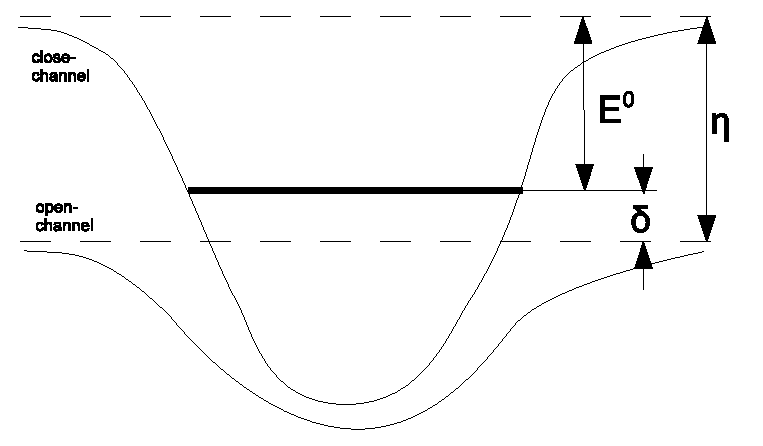
\includegraphics[width=.50\textwidth]{image/FeshbachPotential}
	\caption{Feshbach Resonance Potential\label{fig:FeshbachPotential}}	
\end{figure}

The gap equations are 
\begin{subequations}\label{eq:20100909:fullgap}
\begin{gather}
\frac{2F_{\vk}}{\sqrt{1-4 F_{\vk}^2-4 G_{\vk}^2}} \xi^{ab}_{\vk}+\frac{8 F_{\vk} G_{\vk}^2}{\sqrt{1-4 F_{\vk}^2-4 G_{\vk}^2} \left(1+\sqrt{1-4 F_{\vk}^2-4 G_{\vk}^2}\right)^2}\eta+U_{\vk\vk'}F_{\vk'}+Y_{\vk\vk'}G_{\vk'}=0
\label{eq:20100909:fullgapa}\\
\frac{2G_{\vk}}{\sqrt{1-4 F_{\vk}^2-4 G_{\vk}^2}} \xi^{ac}_{\vk}-\frac{8 F_{\vk}^{2} G_{\vk}}{\sqrt{1-4 F_{\vk}^2-4 G_{\vk}^2} \left(1+\sqrt{1-4 F_{\vk}^2-4 G_{\vk}^2}\right)^2}\eta+V_{\vk\vk'}G_{\vk'}+Y_{\vk\vk'}F_{\vk'}=0
\label{eq:20100909:fullgapb}
\end{gather}
\end{subequations}
where $\eta=\epsilon^{ac}_{\vk}-\epsilon^{ab}_{\vk}$ is the bare Zeeman energy difference and is large than most energy scale, $E_{F}$.  It should be in the order of binding energy of the close-channel bound state.   

The number equation is (see footnote (\ref{foot:20100909:sgn}) for $\sgn_{k}$)
\begin{equation}\label{eq:20100909:number}
N=\sum_{\vk}(v_{\vk}^{2}+w_{\vk}^{2})=\sum_{\vk}\frac{1}{2} \left(1-\sgn_{k}\sqrt{1-4 F_{\vk}^2-4 G_{\vk}^2}\right)
\end{equation} 


\subsection{Approximate close-channel with bound-state level}
It is energetically very disadvantageous to diviate from the resonant bound state, furthermore, it is very small in k-space as the bound-state is relatively small.  Therefore, as the first order approximation, we drop the second term and the denominator in the first term of the second equation (close-channel) of \eef{eq:20100909:fullgap}\footnote{ This is certainly OK for he BEC end where $F_{k}\ll1$ all the time.  It is less satisfactory, might be problematic,  when $F_{k}$ is close to maximum $\nth2$, this happens around Fermi energy in BCS limit, but the approximation is still OK for other places. So at least for bulk of the region of $G_{\vk}$ satisfies \eef{eq:20100915:gapb}}.  In the first equation, we drop the factor $\left(1+\sqrt{1-4 F_{\vk}^2-4 G_{\vk}^2}\right)^2$ in the second term for easier calculation, (no strong reason yet), the second term is relatively minor comparing to the first. We write down the approximated equations
\begin{subequations}\label{eq:20100915:gap}
\begin{gather}\label{eq:20100915:gapa}
\frac{2F_{\vk}}{\sqrt{1-4 F_{\vk}^2-4 G_{\vk}^2}} (\xi^{ab}_{\vk}+  G_{\vk}^2\eta)+U_{\vk\vk'}F_{\vk'}+Y_{\vk\vk'}G_{\vk'}=0\\
\label{eq:20100915:gapb}
{2G_{\vk}}(\xi^{ab}_{\vk}+\eta)+V_{\vk\vk'}G_{\vk'}+Y_{\vk\vk'}F_{\vk'}=0
\end{gather}
\end{subequations}
If $G_{\vk}=\alpha\phi^{0}_{\vk}$ as $\phi_{\vk}^{0}$ is the solution for the isolated close-channel \sch.  
\begin{equation}\label{eq:20100915:twobody}
{2\phi^{0}_{\vk}}(\epsilon_{\vk})+V_{\vk\vk'}\phi^{0}_{\vk'}=-2E^{0}\phi^{0}_{\vk'}
\end{equation}
\eef{eq:20100915:gapb} becomes
\begin{equation}
G_{\vk}=\frac{Y_{\vk\vk'}F_{\vk'}}{2(E^{0}-\eta+\mu)}
\end{equation}
Plug this back into the last term of \eef{eq:20100915:gapa}, we have 
\begin{equation}
\frac{2F_{\vk}}{\sqrt{1-4 F_{\vk}^2-4 G_{\vk}^2}} (\xi^{ab}_{\vk}+  G_{\vk}^2\eta)+U_{\vk\vk'}F_{\vk'}+\frac{Y_{\vk\vk'}Y_{\vk'\vk''}}{2(E^{0}-\eta+\mu)}F_{\vk''}=0
\end{equation}
Now considering the last two terms has weak dependecy in low k, we can set 
\begin{equation}\label{eq:20100915:gap1}
\frac{2F_{\vk}}{\sqrt{1-4 F_{\vk}^2-4 G_{\vk}^2}} \xi^{ab}_{\vk}+  G_{\vk}^2\eta)\equiv\Delta_{\vk}=-(U_{\vk\vk'}F_{\vk'}+\frac{Y_{\vk\vk'}Y_{\vk'\vk''}}{2(E^{0}-\eta+\mu)}F_{\vk''}
\end{equation}
We can express $F_{\vk}$ according to $\Delta_{\vk}$,  (ignore the higher order of $G_{\vk}$)
\begin{equation}\label{eq:20100915:F}
F_{\vk}=\frac{\Delta_{\vk}}2\sqrt{\frac{(1-4G_{\vk}^{2})}{(\xi^{ab}_{\vk}+  G_{\vk}^2\eta)^{2}+\Delta_{\vk}^{2}}}
\end{equation}
Put it back into the second half of gap equation (\ref{eq:20100915:gap1}), 
\begin{equation}\label{eq:20100915:onechannel}
\Delta_{\vk}=-\sum_{\vk'}\br{U_{\vk\vk'}+\frac{Y_{\vk\vk''}Y_{\vk''\vk'}}{2(E^{0}-\eta+\mu)}}\frac{\Delta_{\vk}}2\sqrt{\frac{(1-4G_{\vk}^{2})}{(\xi^{ab}_{\vk}+  G_{\vk}^2\eta)^{2}+\Delta_{\vk}^{2}}}
\end{equation}


\subsection{Two effects of narrow resonance}
There are two possibilities for narrow resonance:  
\begin{enumerate}
\item Pauli exclusion for three species, where the close-channel weight is large.  
\item Fermi energy is larger than the width that scattering amplitude (NOT $a_{s}$) changes the sign.  Therefore $a_{s}$ is no longer a good indicator for the interaction.  However, it might still be OK to take $a_{s}$ simply as the quantity introduced by renormalization.   This has been explored by several papers already \cite{NarrowJensen1,NarrowJensen,GurarieNarrow}.  
\end{enumerate}
Four species case can fall into narrow resonance in  the second sense.  \cite{NarrowJensen1,NarrowJensen} uses the single-channel approach but a T-matrix with effective range $r_{0}$, the narrow resonance is $r_{0}k_{F}\ll1$.  In \cite{NarrowJensen}, a single-channel bare interaction is assumed and (unnormalized) gap, number equations  are  solved numerically with different interaction parameters corresponding to different effective ranges. The result is some small corrections in gap, chemical potential...   It is not a two-channel treatment.  


\subsection{Narrow Resonance}
In narrow resonance, Fermi sea is deep and only part of the fermi sea (strongly) interacts/resonants with the close-cannel bound-state.   \index{Feshbach Resonance!Narrow}
\begin{figure}[hhtb]
	\centering
	         \subfloat[$\delta>E_{F}$]{\label{fig:narrowFR:aboveSea}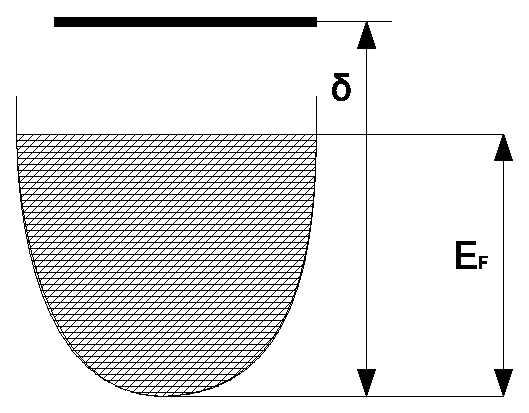
\includegraphics[width=.20\textwidth]{image/narrowFR2.eps}}\quad
		\subfloat[$E_{F}>\delta>0$]{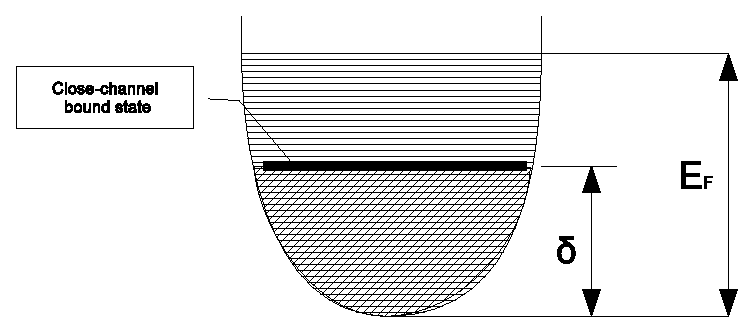
\includegraphics[width=.30\textwidth]{image/narrowFR.eps}\label{fig:narrowFR:inSea}}\quad
		\subfloat[$\delta<0$]{\label{fig:narrowFR:belowSea}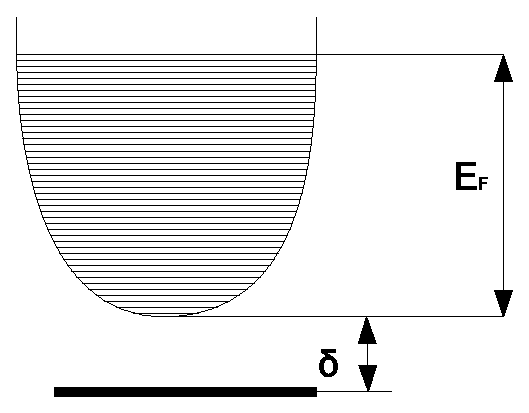
\includegraphics[width=.20\textwidth]{image/narrowFR3.eps}}
	{\caption{Narrow Resonance\label{fig:narrowFR}}
	\parbox{0.7\textwidth}{\small{In fact, in Fig. \subref{fig:narrowFR:inSea} chemical potential would be close to the close-channel bound state level (besides small shift due to open-channel intra-channel coupling) and ``Fermi sea'' above is likely empty. }}}
\end{figure}
Fig. (\ref{fig:narrowFR}).  Here the zero-energy T-matrix is less  physically relevant than those with finite $T(E_{F}-\delta)$.  The more commonly used s-wave scattering length $a_{s}(E)$ likely changes sign within Fermi sea.  $T(E)$ dose not depends on $a_{s}(E)$, but also on effective range $r_{0}$.  

Here BCS/BEC extremes are subtle in the meaning.  If that refers to close-channel bound-state above or below Fermi sea and the interaction is necessarily small as the condition for narrow resonance, they are not very interesting by definition.  When the close-channel bound-state is below zero, most fermions are in close-channel bound-state.  It is BEC of molecules and molecules are mostly in close-channel. When the level is above the Fermi sea, it is fairly far from zero and actually only open-channel fermions near Fermi surface feel relatively strong attraction and they are in BCS.  The more interesting part where it sits in the Fermi sea is always the  case in middle.  

\subsection{Chemical potential}
\emph{Chemical potential is determined in different ways between narrow or broad resonance.  }In broad case, it is determined mostly by open-channel \eef{eq:20100915:gapa}; in narrow case, chemical potential is determined by close-channel, where the close-channel bound-state level sits relative to Fermi sea.  In the extreme narrow case (without open-channel interaction as \cite{GurarieNarrow}), the level is exactly where chemical potential sits, cutting Fermi sea, depleting everything above in open-channel and putting them into close-channel.   

By correcting all equations in previous few sections and put the chemical potential $\mu$ in the proper position, we can see the narrow/broad resonance even in the four species case.  In Eq. (\ref{eq:20100915:t0}-\ref{eq:20100915:tk}), there are two many-body effects: $\sqrt{1-4G_{\vk}^{2}}$ from three-species Pauli exclusion; chemical potential in detuning term $E^{0}-\eta+\mu$, which is common in either three or four-species case.  And the later reduces to $\mu=0$ \footnote{In BEC side, $\mu<0$ and is controlled by mostly two-body attraction.  But that is not proper for real two-body limit, which should be $\mu=0$.}in zero-density which is two-body case. 

Imaging we start fairly far away from resonance (BCS side, $\delta=\eta-E^{0}>0$), and increase the density, in the beginning, $\mu$ is negligible, and inter-channel coupling term $\frac{Y_{\vk\vk''}Y_{\vk''\vk'}}{2(E^{0}-\eta+\mu)} $ is small; as $\mu$  increases, $-(\delta-\mu)$ gets closer and closer to zero, and this terms increases until the part of the Fermi sea gets into resonance.  





\subsection{Renormalization of gap equation}
At low k, $\Delta_{\vk}$ has weak dependency on k and we can take $\Delta_{\vk'}$ out of the summation,  then go through the same procedure as in \cite{Leggett,Fetter} to renormalize the equation. There are more than one options to renormalize gap equation \eef{eq:20100915:onechannel}.  The part that needs to be renormalized out is  high energy summation of $\sqrt{\frac{(1-4G_{\vk'}^{2})}{{(\xi^{ab}_{\vk}+  G_{\vk}^2\eta)^{2}+\Delta_{\vk}^{2}}}}$, it approaches $\nth{\epsilon_{\vk}}$ in high energy.  Several sightly different physical quantities have the summation of the same high energy limit.  
\begin{enumerate}

\item We can also notice that $G_{\vk}\rightarrow0$ at high energy.  So we can simply takes the normal \emph{zero-energy} T-matrix with detuning related to chemical potential.  
\begin{equation}\label{eq:20101004:renormGap1}
\nth{{t_{0}}(\mu)}=\sum_{\vk}
\br{\nth{\epsilon_{\vk}}-\frac{\sqrt{(1-4G_{\vk}^{2})}}{\sqrt{{(\xi^{ab}_{\vk}+  G_{\vk}^2\eta)^{2}+\Delta_{\vk}^{2}}}}}
\end{equation} 
\begin{gather}
{t_{0}}(\mu)=\br{1-\tilde{U}\tilde{ K}}^{-1}\tilde{U}\label{eq:20101004:t01}\\
\tilde{U}_{\vk\vk'}=\nth{2} \br{U_{\vk\vk'}+\frac{Y_{\vk\vk''}Y_{\vk''\vk'}}{2(E^{0}-\eta+\mu)}}\label{eq:20101004:tu1}\\
{K}=\nth{\epsilon_{\vk}}\delta_{\vk\vk'}\label{eq:20101004:tk1}
\end{gather}
Here Eqs. (\ref{eq:20101004:t01}-\ref{eq:20101004:tk1}) follows the same two-body formula for zero-energy T-matrix element.  However, the detuning is shifted by a many-body quantity $\mu$ that should be determined by solving gap equation with numberequation.    
\item  Alternatively, we notice that $\xi_{\vk}=\epsilon_{\vk}-\mu$, high energy limit can also be written as 
$\nth{\epsilon_{\vk}-\mu}$.  This leads to the T-matrix at energy $\mu$, the same detuning as before.  
\begin{equation}\label{eq:20101004:renormGap2}
\nth{{t_{\mu}}(\mu)}=\sum_{\vk}
\br{\nth{\epsilon_{\vk}-\mu}-\frac{\sqrt{(1-4G_{\vk}^{2})}}{\sqrt{{(\xi^{ab}_{\vk}+  G_{\vk}^2\eta)^{2}+\Delta_{\vk}^{2}}}}}
\end{equation} 
\begin{gather}
{t_{\mu}}(\mu)=\br{1-\tilde{U}\tilde{ K}}^{-1}\tilde{U}\label{eq:20101004:t02}\\
\tilde{U}_{\vk\vk'}=\nth{2} \br{U_{\vk\vk'}+\frac{Y_{\vk\vk''}Y_{\vk''\vk'}}{2(E^{0}-\eta+\mu)}}\label{eq:20101004:tu2}\\
{K}=\nth{\epsilon_{\vk}-\mu}\delta_{\vk\vk'}\label{eq:20101004:tk2}
\end{gather}
The advantage of this is that introduce the effective range $r_{0}$ for finite energy T-matrix. 
\end{enumerate}


It seems the second method would be the most convenient choice.  
\subsection{Pauli exclusion factor  $\sqrt{(1-4G_{\vk'}^{2})}$ }
It seems that numerous Gap equations above has the Pauli-exclusion factor $\sqrt{(1-4G_{\vk'}^{2})}$.  Generally, 
\begin{equation}
G_{k=0}^{2}\sim{\frac{N_{close}}{N_{0}}\frac{r_{close}^{3}}{a_{0}^{3}}}
\end{equation}
where $r_{close}$ is close-channel molecule size, $N_{0}$ is the total number of fermions, $N_{close}$ is the number in close-channel, $a_{0}$ is the average particle distance.  This quantity is related the detail of close-channel bound-state.  We should relate it to some experimental available quantities.  In the above expression, factor $r_{close}^{3}/a_{0}^{3}$ relates to the two-body physics, while $N_{close}/N_{0}$ relates to many-body physics which probably needs to be solved consistently with the many-body equation .  

\subsection{More on chemical potential shift for detuning}
Let us image a sweep of $\delta$ from BCS end.  At the very BCS end, $\delta$ is positive and large than $\mu\approx{}E_{F}$ (Fig. \ref{fig:narrowFR:aboveSea}). Resonant term in interaction is relatively small and close-channel weight is small too.  We are very well in the  weak-attraction (slightly enhanced by resonance) BCS-like state in open-channel.  However, the detuning is shifted by $\mu\approx{}E_{F}$, so the resonance is reached earlier, and the larger the density, the earlier it does.  

As the detuning gets close to Fermi surface, chemical potential decreases from $E_{F}$. For narrow resonance, $E_{F}$ is large than the resonance energy scale.  The resonance reaches probably before detuning reaches Fermi surface.  If we ignore the shift due to open-channel intra-channel coupling for the moment, the resonance is very close at the point where $\delta=E_{F}$.  After $\delta$ drops into Fermi sea (Fig. \ref{fig:narrowFR:inSea}), chemical potential $\mu$ tracks the close-channel bound-state closely and the denominator of resonant term $-(\delta-\mu)$ keeps very small, and in some sense, the Feshbarch resonance is enhanced by the many-body  physics.  Open-channel still has energy advantages below $\mu$, so both channels are important.  

After $\delta$ drops below zero (Fig. \ref{fig:narrowFR:belowSea}), chemical potential still tracks $\delta$, but now most weight is in close-channel and the bound-state is mostly made of close-channel.  

\subsection{Number equation}
For number equation \eef{eq:20100909:number}, more approximation can be made in Feshbach resonance.  Close-channel component $G_{k}$ is much extended in k-space due to the tight-binding, and $F_{k}$ is significant up to the order of Fermi energy $E_{F}$.  It seems OK to assume that most weight of close-channel lies beyond $E_{F}$, so when $\epsilon_{k}\gg{E_{F}}$, the integrand becomes simply $G_{k}^{2}$, the summation gives $N_{close}$.  Therefore we have 
\begin{equation}\label{eq:20100909:number}
N_{open}=\sum_{\vk}{}^{'}\frac{1}{2} \left(1-\sgn_{k}\sqrt{1-4 F_{\vk}^2-4 G_{\vk}^2}\right)-G_{\vk}^{2}
\end{equation} 
Here the summation only goes up to the order of $E_{F}$

\subsection{summary}
Now all summation goes in order of Fermi energy $E_F$, so we can replace close-channel component $G_k$ with $G_0=G_{k=0}$
\begin{equation}
F_{\vk}=\frac{\Delta_{\vk}}2\sqrt{\frac{(1-4G_{0}^{2})}{(\epsilon^{ab}_{\vk}-2\mu+  G_{0}^2\eta)^{2}+\Delta_{\vk}^{2}}}
\end{equation}
Gap equation 
\begin{equation}\label{eq:20101004:renormGap1}
\nth{{t_{0}}(\mu)}=\sum_{\vk}
\br{\nth{\epsilon_{\vk}}-\frac{\sqrt{(1-4G_{0}^{2})}}{\sqrt{{(\epsilon^{ab}_{\vk}-2\mu+  G_{0}^2\eta)^{2}+\Delta_{\vk}^{2}}}}}
\end{equation} 
\begin{gather}
{t_{0}}(\mu)=\br{1-\tilde{U}\tilde{ K}}^{-1}\tilde{U}\label{eq:20101004:t01}\\
\tilde{U}_{\vk\vk'}=\nth{2} \br{U_{\vk\vk'}+\frac{Y_{\vk\vk''}Y_{\vk''\vk'}}{2(E^{0}-\eta+\mu)}}\label{eq:20101004:tu1}\\
{K}=\nth{\epsilon_{\vk}}\delta_{\vk\vk'}\label{eq:20101004:tk1}
\end{gather}
Here Eqs. (\ref{eq:20101004:t01}-\ref{eq:20101004:tk1}) follows the same two-body formula for zero-energy T-matrix element.  However, the detuning is shifted by a many-body quantity $\mu$ that should be determined by solving gap equation with number equation.  
And number equation
\begin{equation}\label{eq:20100909:number}
N_{open}=\sum_{\vk}{}^{'}\frac{1}{2} \left(1-\sgn_{k}\sqrt{1-4 F_{\vk}^2-4 G_{0}^2}\right)-G_{0}^{2}
\end{equation} 
These equations have two common variables $\mu$, $\Delta$ as well as two other quantities, $G_0$, $\eta$.  These two quantities relate to  two-body physics and can vary for the same set $\mu$, $\Delta$.  I have not seen the way to convert them into some experimental measurables.  
\section{Number/Gap equations}
\subsection{number equation}
Put \eef{eq:20100915:F} into number equation \eef{eq:20100909:number}, we have\footnote{Here we drop $\sgn_{k}$ as $(\epsilon^{ab}_{\vk}-2\mu+  G_{0}^2\eta)$ takes care of the sign}
\begin{equation}\label{eq:20101011:number}
N=\sum{1-\sqrt{1-4G_{k}^{2}}\frac{(\epsilon^{ab}_{\vk}-2\mu+  G_{\vk}^2\eta)}{{\sqrt{{(\epsilon^{ab}_{\vk}-2\mu+  G_{\vk}^2\eta)^{2}+\Delta^{2}}}}}}
\end{equation}
This equation also requires to take into account that $G_{k}$ approaches 0 at high momentum to be convergent.  
\subsection{typical energy scale}
I calculated $^{6}\text{Li}$'s Fermi energy for density $10^{15}\text{cm}^{-3}$, it is $5\times10^{-28}J$, for Bohr magneton $\mu_{B}=9.27\times10^{-24}\text{J T}^{-1}$, it corresponds magnetic field $B=0.5\times10^{-4}\text{T}=0.5\text{G}$.

\subsection{more on $G_{k}$ and $\eta$}
$\phi^{0}$ the w.f. of two-body close-channel bound state varies in different Feshbach resonance and is a case-specific quantity.  Its property can be lumped into the general two-body Feshbach resonance formula and usually does not matter.  It does matter in narrow resonance problem.  However, this can be simplified if it is a high-energy bound-state, that mostly is outside the potential.  Therefore, most weight of $\phi^{0}$ follows the simple form 
\[
\phi^{0}(r)=C\frac{e^{-\kappa{r}}}{r}
\]
 where $\frac{\hbar^{2}\kappa^{2}}{2m}=E^{0}$ and $\kappa>0$.  $C^{2}=\frac{\kappa}{2\pi}$.  Convert it into k-space
 \begin{equation}\label{eq:20101011:phi}
\phi^{0}_k=\nth{(2\pi)^{\frac32}}\int{d^{3}\vr\phi^{0}(r)e^{-i\vk\cdot\vr}}=\nth{\pi}\frac{\kappa}{k^{2}+\kappa^{2}}
\end{equation}
Now we can estimated $G_{k}^{2}\eta$. $G_{k}=\alpha\phi^{0}_{k}$ where 
\[|\alpha|^{2}<n\sim{E_{F}^{3/2}}\]
\[
\abs{\phi^{0}_{k}}^{2}=\nth{\pi^{2}\kappa^{3}}\sim\nth{(E^{0})^{3/2}}
\]
And $\eta\sim{E^{0}}$, So 
\[
G_{k}^{2}\eta<G_{k=0}^{2}\eta<E_{F}(\frac{E_{F}}{E^{0}})^{1/2}
\]
And we have $E_{F}\ll{E^{0}}$, so this term is much smaller than $\mu\sim{E_{F}}$ in BCS side. For now, we just omit this term.  Considering $G_{k}^{2}\ll1$, we can expand $\sqrt{1-4G_{k}^{2}}$ in \eef{eq:20101011:number} and \eef{eq:20101004:gapS} 
\begin{gather}
\nth{{t_{0}}(\mu)}=\sum_{\vk}
\br{\nth{\epsilon_{\vk}}-\frac{1}{\sqrt{{(\epsilon^{ab}_{\vk}-2\mu)^{2}+\Delta_{\vk}^{2}}}}
+\frac{2\alpha^{2}|\phi^{0}_{k}|^{2}}{\sqrt{{(\epsilon^{ab}_{\vk}-2\mu)^{2}+\Delta_{\vk}^{2}}}}}
\\
N=\sum{1-\frac{(\epsilon^{ab}_{\vk}-2\mu)}{{\sqrt{{(\epsilon^{ab}_{\vk}-2\mu)^{2}+\Delta^{2}}}}}
+2\alpha^{2}|\phi^{0}_{k}|^{2}\frac{(\epsilon^{ab}_{\vk}-2\mu)}{{\sqrt{{(\epsilon^{ab}_{\vk}-2\mu)^{2}+\Delta^{2}}}}}}
\end{gather}
Here $\phi^{0}_{k}$ takes the form in \eef{eq:20101011:phi} and we have an extra quantity $\kappa$ ($E^{0}$), also, we have 
\begin{equation}
\Delta_{\vk}=U_{\vk\vk'}F_{\vk'}+Y_{\vk\vk'}G_{\vk'}\approx\alpha{Y_{\vk\vk'}\phi^{0}_{\vk'}}
\end{equation}
\[\Delta^{2}\approx\alpha^{2}(\Delta^{2})|_{\text{very BEC end}}
\]
Here we can see that $\Delta$ saturates in BEC end where close-channel dominates.  
\bibliography{citation}
\bibliographystyle{amsplain}


\end{document}
